% https://tex.stackexchange.com/questions/119625/mindmap-level-specific-child-distance?rq=1
\documentclass{standalone}
\usepackage{tikz}
\usetikzlibrary{mindmap,trees}

\begin{document}
\resizebox{!}{4 in}{%
   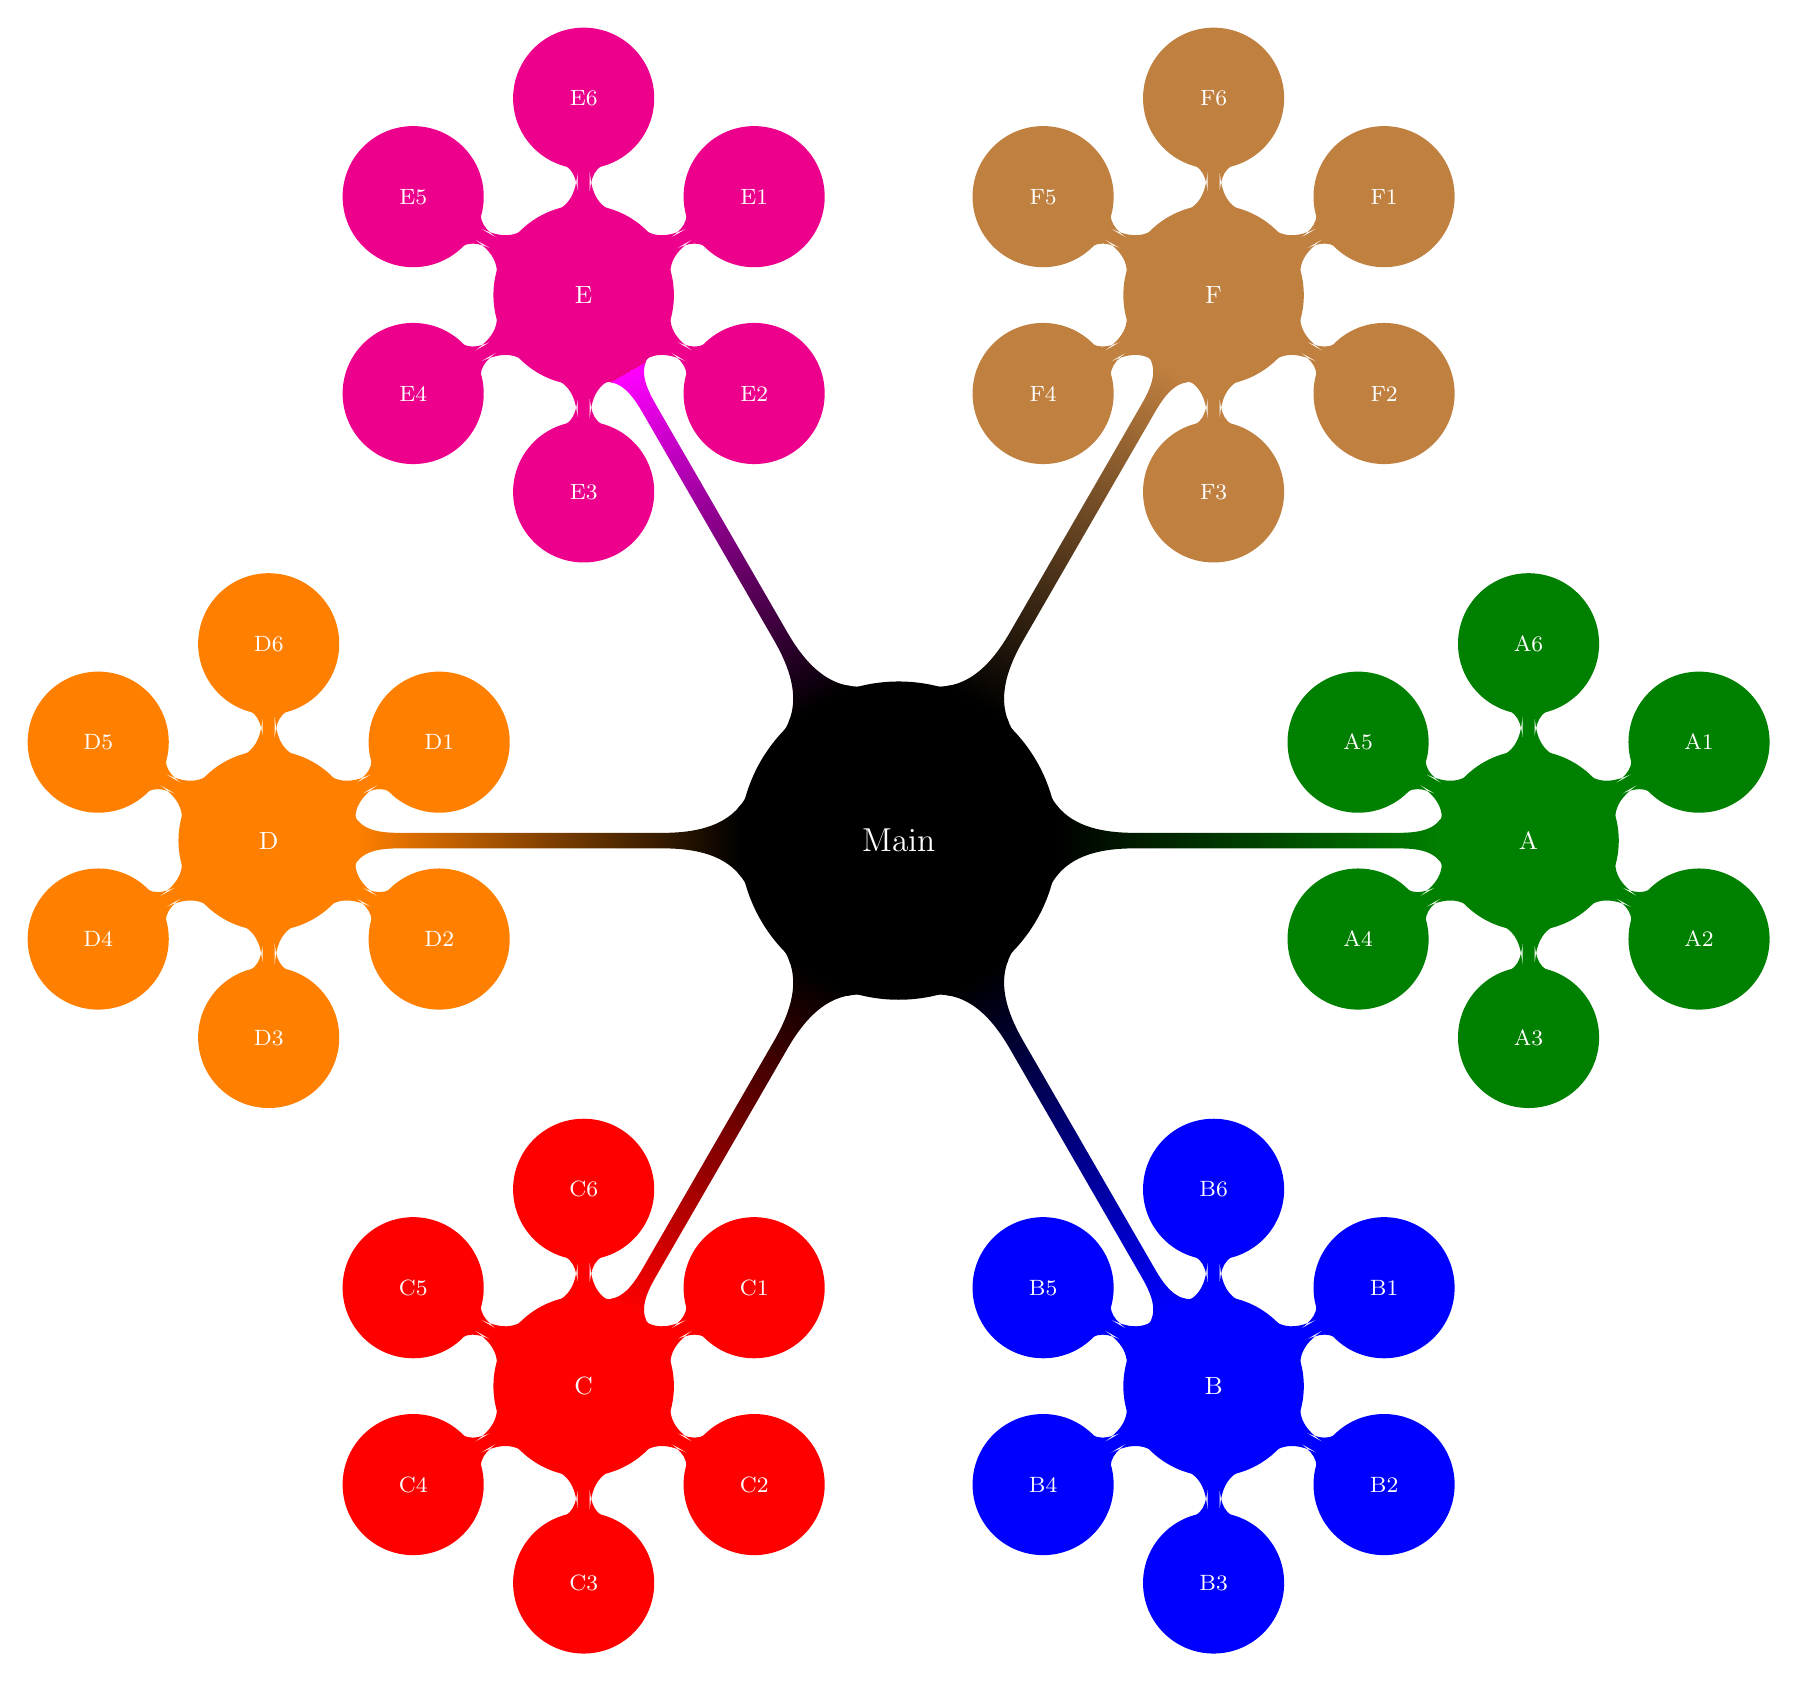
\begin{tikzpicture}
      \path[
         mindmap,
         concept color=black,
         text=white,
         grow cyclic,
         segment length=20cm,
   level 1/.append style={level distance=8cm,sibling angle=60},
   level 2/.append style={level distance=2.5cm},
      ]
      node[concept] {Main}
      [clockwise from=0]
      child[concept color=green!50!black] {%
         node[concept] {A}
         [clockwise from=30]
         child {node[concept] {A1} }
         child {node[concept] {A2} }
         child {node[concept] {A3} }
         child {node[concept] {A4} }
         child {node[concept] {A5} }
         child {node[concept] {A6} }
      }  
      child[concept color=blue] {%
         node[concept] {B}
         [clockwise from=30]
         child {node[concept] {B1} }
         child {node[concept] {B2} }
         child {node[concept] {B3} }
         child {node[concept] {B4} }
         child {node[concept] {B5} }
         child {node[concept] {B6} }
      }
      child[concept color=red] {%
         node[concept] {C}
         [clockwise from=30]
         child {node[concept] {C1} }
         child {node[concept] {C2} }
         child {node[concept] {C3} }
         child {node[concept] {C4} }
         child {node[concept] {C5} }
         child {node[concept] {C6} }
      }
      child[concept color=orange] {%
         node[concept] {D}
         [clockwise from=30]
         child {node[concept] {D1} }
         child {node[concept] {D2} }
         child {node[concept] {D3} }
         child {node[concept] {D4} }
         child {node[concept] {D5} }
         child {node[concept] {D6} }
      }
      child[concept color=magenta] {%
         node[concept] {E}
         [clockwise from=30]
         child {node[concept] {E1} }
         child {node[concept] {E2} }
         child {node[concept] {E3} }
         child {node[concept] {E4} }
         child {node[concept] {E5} }
         child {node[concept] {E6} }
      }
      child[concept color=brown] {%
         node[concept] {F}
         [clockwise from=30]
         child {node[concept] {F1} }
         child {node[concept] {F2} }
         child {node[concept] {F3} }
         child {node[concept] {F4} }
         child {node[concept] {F5} }
         child {node[concept] {F6} }
      };
   \end{tikzpicture}
}
\end{document}